\documentclass[10pt]{article}\usepackage[]{graphicx}\usepackage[]{color}
%% maxwidth is the original width if it is less than linewidth
%% otherwise use linewidth (to make sure the graphics do not exceed the margin)
\makeatletter
\def\maxwidth{ %
  \ifdim\Gin@nat@width>\linewidth
    \linewidth
  \else
    \Gin@nat@width
  \fi
}
\makeatother

\definecolor{fgcolor}{rgb}{0.345, 0.345, 0.345}
\newcommand{\hlnum}[1]{\textcolor[rgb]{0.686,0.059,0.569}{#1}}%
\newcommand{\hlstr}[1]{\textcolor[rgb]{0.192,0.494,0.8}{#1}}%
\newcommand{\hlcom}[1]{\textcolor[rgb]{0.678,0.584,0.686}{\textit{#1}}}%
\newcommand{\hlopt}[1]{\textcolor[rgb]{0,0,0}{#1}}%
\newcommand{\hlstd}[1]{\textcolor[rgb]{0.345,0.345,0.345}{#1}}%
\newcommand{\hlkwa}[1]{\textcolor[rgb]{0.161,0.373,0.58}{\textbf{#1}}}%
\newcommand{\hlkwb}[1]{\textcolor[rgb]{0.69,0.353,0.396}{#1}}%
\newcommand{\hlkwc}[1]{\textcolor[rgb]{0.333,0.667,0.333}{#1}}%
\newcommand{\hlkwd}[1]{\textcolor[rgb]{0.737,0.353,0.396}{\textbf{#1}}}%
\let\hlipl\hlkwb

\usepackage{framed}
\makeatletter
\newenvironment{kframe}{%
 \def\at@end@of@kframe{}%
 \ifinner\ifhmode%
  \def\at@end@of@kframe{\end{minipage}}%
  \begin{minipage}{\columnwidth}%
 \fi\fi%
 \def\FrameCommand##1{\hskip\@totalleftmargin \hskip-\fboxsep
 \colorbox{shadecolor}{##1}\hskip-\fboxsep
     % There is no \\@totalrightmargin, so:
     \hskip-\linewidth \hskip-\@totalleftmargin \hskip\columnwidth}%
 \MakeFramed {\advance\hsize-\width
   \@totalleftmargin\z@ \linewidth\hsize
   \@setminipage}}%
 {\par\unskip\endMakeFramed%
 \at@end@of@kframe}
\makeatother

\definecolor{shadecolor}{rgb}{.97, .97, .97}
\definecolor{messagecolor}{rgb}{0, 0, 0}
\definecolor{warningcolor}{rgb}{1, 0, 1}
\definecolor{errorcolor}{rgb}{1, 0, 0}
\newenvironment{knitrout}{}{} % an empty environment to be redefined in TeX

\usepackage{alltt}
\usepackage{graphicx, verbatim}
\usepackage{amsmath}
\usepackage{amssymb}
\usepackage{amscd}
\usepackage{lipsum}
\usepackage{todonotes}
\usepackage[tableposition=top]{caption}
\usepackage{ifthen}
\usepackage[utf8]{inputenc}
\usepackage{graphicx}
\usepackage{caption}
\setlength{\textwidth}{6.5in} 
\setlength{\textheight}{9in}
\setlength{\oddsidemargin}{0in} 
\setlength{\evensidemargin}{0in}
\setlength{\topmargin}{-1.5cm}
\setlength{\parindent}{0cm}
\usepackage{setspace}
\usepackage{float}
\usepackage{amssymb}
\usepackage[utf8]{inputenc}
\usepackage{fancyhdr}
\usepackage{tabularx}

\usepackage{hyperref}
\hypersetup{
  colorlinks   = true, %Colours links instead of ugly boxes
  urlcolor     = blue, %Colour for external hyperlinks
  linkcolor    = blue, %Colour of internal links
  citecolor   = red %Colour of citations
}

%\fancyhf{}
\rfoot{Andrew Tait \thepage}
\singlespacing
\usepackage[affil-it]{authblk} 
\usepackage{etoolbox}
\usepackage{lmodern}


% Notice the following package, it will help you cite papers
\usepackage[backend=bibtex ,sorting=none]{biblatex}
\bibliography{references}

\begin{filecontents*}{references.bib}

\end{filecontents*}
\IfFileExists{upquote.sty}{\usepackage{upquote}}{}
\begin{document}


\title{\LARGE Coursework  \\ Data Science Development (CMM535)}

\author{Andrew Tait, \textit{\href{1504693@rgu.ac.uk}{1504693@rgu.ac.uk}}}
\maketitle
% \begin{flushleft} \today \end{flushleft} 
\noindent\rule{16cm}{0.4pt}
%\underline{\hspace{3cm}
\ \\
%\thispagestyle{empty}

\section{Research}

[your text goes here]
The paper that was chosen for this work is \cite{6779381}. The authors provided a full review on different streaming algorithms and methos that handle concept drfit?. Below is a review of this paper that includes problem statement, related work and methods applied.\\

\textcolor{blue}{\textit{Notice how I cited the paper, and how does it appear in the document, to do so, you need to have a file in your working director (references.bib), this file simply contains the bibtext items for the papers you chose. These BibTex items are often avaiable to download from publishers website, see Figure~\ref{fig1}}}
\subsection{Problem Statement}
What is this paper about? your text goes here, your text goes here your text goes here your text goes here your text goes here your text goes here your text goes here

\subsection{Relevant Work}
[your text goes here your text goes here your text goes here your text goes here your text goes here your text goes here your text goes here your text goes here your text goes here your text goes here your text goes here your text goes here your text goes here your text goes here]
\subsection{Methods}
[your text goes here your text goes here your text goes here your text goes here your text goes here your text goes here your text goes here your text goes here your text goes here your text goes here your text goes here your text goes here your text goes here your text goes here]
\subsection{Results}
[your text goes here your text goes here your text goes here your text goes here your text goes here your text goes here your text goes here your text goes here your text goes here your text goes here your text goes here your text goes here your text goes here your text goes here]
\subsection{Conclusion}

[your text goes here your text goes here your text goes here your text goes here your text goes here your text goes here your text goes here your text goes here your text goes here your text goes here your text goes here your text goes here your text goes here your text goes here]




\section {Data Streams}

The dataset that has been chosen for this part of the course work is IRIS. This is available on the UCI repository. The set was chosen because of .... It proves to be a good set for evaluating 'x' methods .... 

\subsection{Data Exploration}

Explore the dataset as required by the course work. Discuss, visualise, summarise ... Make sure utilise what you have learnt in the class .... Presenting results is important. Here are some expampoles.... \\

It is a good practice to separate the code from the results, this makes the document more readable and easier to reproduce. Here is an example, where I want to show the class distribution in my dataset.

% notice that eval=FALSE will show the code but not execute it, also notice that the comment=NA will cause the # to disappear from the output. 

\begin{knitrout}
\definecolor{shadecolor}{rgb}{0.969, 0.969, 0.969}\color{fgcolor}\begin{kframe}
\begin{alltt}
\hlkwd{table}\hlstd{(iris}\hlopt{$}\hlstd{Species)}
\end{alltt}
\end{kframe}
\end{knitrout}

\begin{knitrout}
\definecolor{shadecolor}{rgb}{0.969, 0.969, 0.969}\color{fgcolor}\begin{kframe}
\begin{verbatim}

    setosa versicolor  virginica 
        50         50         50 
\end{verbatim}
\end{kframe}
\end{knitrout}

\textbf{Tables}: If you want to show results in a table format, the package \textcolor{blue}{xtable} is very useful. Here is a an example: suppose you want to show the head of iris data, a simple way is to do the following: 

\begin{knitrout}
\definecolor{shadecolor}{rgb}{0.969, 0.969, 0.969}\color{fgcolor}\begin{kframe}
\begin{alltt}
\hlkwd{head}\hlstd{(iris)}
\end{alltt}
\end{kframe}
\end{knitrout}

\begin{knitrout}
\definecolor{shadecolor}{rgb}{0.969, 0.969, 0.969}\color{fgcolor}\begin{kframe}
\begin{verbatim}
  Sepal.Length Sepal.Width Petal.Length Petal.Width Species
1          5.1         3.5          1.4         0.2  setosa
2          4.9         3.0          1.4         0.2  setosa
3          4.7         3.2          1.3         0.2  setosa
4          4.6         3.1          1.5         0.2  setosa
5          5.0         3.6          1.4         0.2  setosa
6          5.4         3.9          1.7         0.4  setosa
\end{verbatim}
\end{kframe}
\end{knitrout}

This is fine, but sometimes you want to produce  the results in a table-format at a better standard. See the code below. Often, I won't show the code below, nor make it executable (i.e. set eval=FALSE). Instead, run the commands below in the console, then copy the resulting latex code from consle and paste it below, and add caption and label as shown below

\begin{knitrout}
\definecolor{shadecolor}{rgb}{0.969, 0.969, 0.969}\color{fgcolor}\begin{kframe}
\begin{alltt}
\hlcom{# load package }
\hlkwd{library}(xtable)
\hlcom{# run the following command in the console}
\hlkwd{print}(\hlkwd{xtable}(\hlkwd{head}(iris))
\hlcom{# copy the resulting latex code from consle and paste it below}
\hlcom{# Add caption and label as shown below}
\end{alltt}
\end{kframe}
\end{knitrout}

% latex table generated in R 3.3.0 by xtable 1.8-2 package
% Fri Mar  2 11:56:14 2018
\begin{table}[ht]
\centering
\caption{Iris Data}
\begin{tabular}{rrrrrl}
  \hline
 & Sepal.Length & Sepal.Width & Petal.Length & Petal.Width & Species \\ 
  \hline
1 & 5.10 & 3.50 & 1.40 & 0.20 & setosa \\ 
  2 & 4.90 & 3.00 & 1.40 & 0.20 & setosa \\ 
  3 & 4.70 & 3.20 & 1.30 & 0.20 & setosa \\ 
  4 & 4.60 & 3.10 & 1.50 & 0.20 & setosa \\ 
  5 & 5.00 & 3.60 & 1.40 & 0.20 & setosa \\ 
  6 & 5.40 & 3.90 & 1.70 & 0.40 & setosa \\ 
   \hline
\end{tabular}
\label{tab1}
\end{table}

The good thing about the above approach is you can always refer to the table in your document. For example 'As can be seen in Table~\ref{tab1},...'

\textbf{Figures:} are important part of your analysis, and also good way to give insight about the dataset you are working with. You will use packages like \textit{ggplot2} to produce some visuals. Lets start with a simple example to show how to present your visuals in the report with proper labels and captions. Remember, I need to see the code the produced the figure as well. \\

Suppose, I just want to create a plot that shows the relation between Petal width and length and map the colour and shape to the Species (class label in my dataset). \\

First, I will write my code, but notice that my chunk definition is set as follows\\ \textit{(<<warning=FALSE,message=FALSE,eval=FALSE>>=)}, I set warning and message to FALSE, because I don't want these warnings/ messages to appear in my final output. 


\begin{knitrout}
\definecolor{shadecolor}{rgb}{0.969, 0.969, 0.969}\color{fgcolor}\begin{kframe}
\begin{alltt}
\hlkwd{library}\hlstd{(ggplot2)}

\hlstd{p} \hlkwb{<-} \hlkwd{ggplot}\hlstd{(iris,} \hlkwd{aes}\hlstd{(}\hlkwc{x}\hlstd{=Petal.Length,}
                      \hlkwc{y} \hlstd{= Petal.Width,}\hlkwc{color}\hlstd{=Species) )}
\hlstd{p} \hlkwb{<-} \hlstd{p}\hlopt{+} \hlkwd{geom_point}\hlstd{(}\hlkwd{aes}\hlstd{(}\hlkwc{shape}\hlstd{=Species))}
\hlstd{p} \hlkwb{<-} \hlstd{p} \hlopt{+} \hlkwd{xlab}\hlstd{(}\hlstr{'Petal Length'}\hlstd{)}
\hlstd{p} \hlkwb{<-} \hlstd{p} \hlopt{+} \hlkwd{ylab}\hlstd{(}\hlstr{'Petal Width'}\hlstd{)}
\hlstd{p} \hlkwb{<-} \hlstd{p} \hlopt{+} \hlkwd{theme_bw}\hlstd{()}
\hlstd{p}
\end{alltt}
\end{kframe}
\end{knitrout}

Make sure that your code is running, and once everything is OK, then you need to insert the above code within a Latex code used to insert images (check the .rnw file to see how we achieved this). Again, remember the caption and the label which allows you to refer to this figure from anywhere in your document (Figure~\ref{fig1}). Notice the header of the chunk code in the \textit{.rnw} file. 

\begin{figure}[H]
\begin{center}

\begin{knitrout}
\definecolor{shadecolor}{rgb}{0.969, 0.969, 0.969}\color{fgcolor}
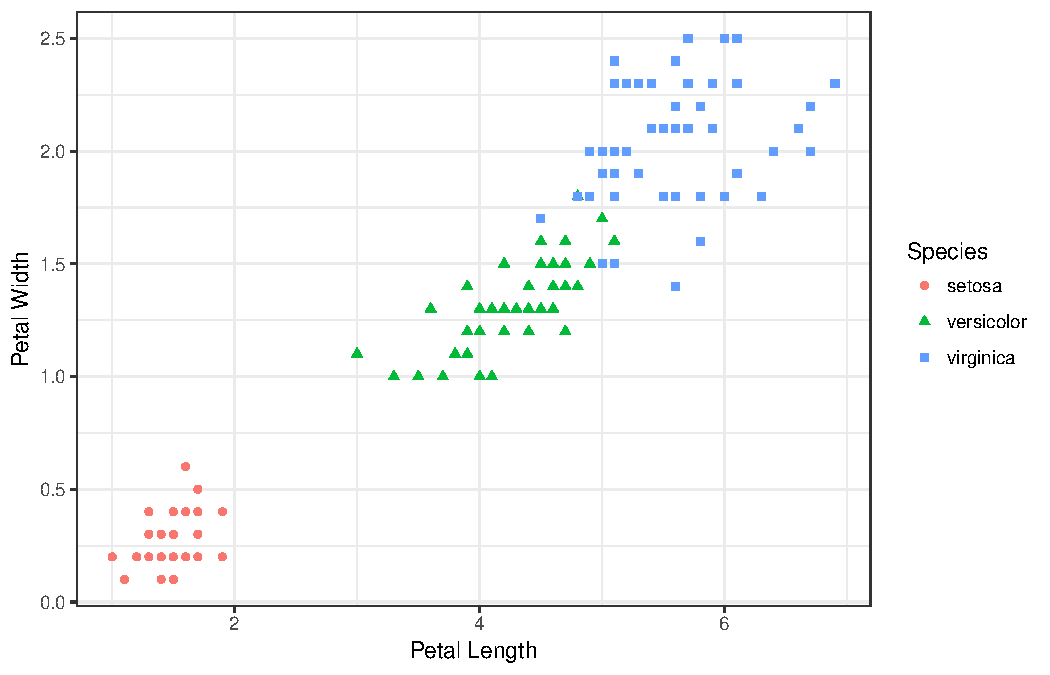
\includegraphics[width=.76\linewidth]{figure/unnamed-chunk-7-1} 

\end{knitrout}
\caption {Petal Length /Width per species in IRIS set}
\label{fig1}
\end {center}
\end {figure}




\subsection{Build Classifier}


Complete this part as required by the coursework sheet. Again, be clear, visuals always helps in communicating results. Justify your choices and explain your methods. 




\subsection{Build Stream Classifier}

Same as above. Complete this part as required by the coursework sheet. Again, be clear, visuals always helps in communicating results. Justify your choices and explain your methods. 




\section {Text Classification}

Same as above. Complete this part as required by the coursework sheet. Again, be clear, visuals always helps in communicating results. Justify your choices and explain your methods. 


\subsection{Preprocessing}

Record, explain and justify your appraoch. Record, explain and justify your appraoch. 
Record, explain and justify your appraoch. Record, explain and justify your appraoch.Record, explain and justify your appraoch.Record, explain and justify your appraoch.Record, explain and justify your appraoch.Record, explain and justify your appraoch. 
Record, explain and justify your appraoch. 


\subsection{Text Analysis}

Record, explain and justify your appraoch.Complete this part as required by the coursework sheet. Again, be clear, visuals always helps in communicating results. Justify your choices and explain your methods. 



\subsection{Text Classification}

Use one of the ‘R’ packages to build a classifier that classifies the tweets as leave tweet or remain tweets. 

Complete this part as required by the coursework sheet. Again, be clear, visuals always helps in communicating results. Justify your choices and explain your methods. 


\section{Reproducing Results}

You don't need to have a section called \textbf{Reproducing Results}, your report itself will be the answer for this section. 


% Clear the page and starte a new page for references 

\clearpage
% The title for the reference section is called References 

\section{References}\label{pubs}

\printbibliography[heading =none]


\clearpage


\end{document}
